\documentclass[12pt, titlepage, oneside]{article}

\usepackage[margin=0.5in]{geometry}

\usepackage{siunitx, booktabs, amsmath, enumitem, pdfpages,mathrsfs,tabularx,caption, graphicx, pgfplots, textcomp,wrapfig, commath, svg}

\usepackage{amssymb}

\usepackage{parskip}

\usepackage[siunitx]{circuitikz}
\sisetup{detect-weight=true, detect-family=true}

\setlength\parindent{0pt}

\let\oldhat\hat
\let\oldvec\vec
\newcommand{\cross}{\bm{\times}}
\renewcommand{\hat}[1]{\oldhat{\mathbf{#1}}}

\usepackage{bm}
\renewcommand{\vec}[1]{\oldvec{\bm{#1}}}
\renewcommand{\hat}[1]{\oldhat{\bm{#1}}}
\renewcommand{\b}[1]{\textbf{#1}}

\newcommand{\de}[1]{\noindent\fbox{\parbox{\textwidth}{#1}}}

\newcommand{\be}{\begin{equation*}}
\newcommand{\ee}{\end{equation*}}

\begin{document}

\section{Marginal Probability Distribution}


Let $X$ and $Y$ be random variables whose distribution can be obtained by summing or integrating over all relevant values of the other random variable. This provides the \b{marginal} p.m.f or p.d.f 
\begin{align}
f_{X}(x) = \sum_y f_{XY}(x,y) \enspace f_Y(y) = \sum_x f_{XY}(x,y)\\
f_X(x) = \int_y f_{XY}(x,y) \, dy \enspace f_Y = \int_x f_{XY}(x,y) \, dx
\end{align}

\de{
\b{Example 5.3} 

Let the columns $X$ be the number of bars of service. Let the rows $Y$ be the response time from cell towers

\begin{center}
\begin{tabular}{c|ccc}
	  & 1    &  2   &  3 \\ \toprule
	4 & 0.15 & 0.1  & 0.05 \\
	3 & 0.02 & 0.1  & 0.05 \\
	2 & 0.02 & 0.03 & 0.2 \\
	1 & 0.01 & 0.02 & 0.25 \\
	\end{tabular}

\end{center}
From this we see:
\begin{center}
\begin{tabular}{cc}
	$x$ & $f_X(x)$ \\ \toprule
	1 & 0.15 + 0.02 + 0.02 + 0.01\\
	2 & 0.1 + 0.1 + 0.03 + 0.02 \\
	3 & 0.05 + 0.05 + 0.2 + 0.25\\
	
\end{tabular}
\end{center}
and 
\begin{center}
\begin{tabular}{cc}
$y$ & $f_Y(y)$ \\ \toprule
	1 & 0.01 + 0.02 + 0.25\\
	2 & 0.02 + 0.03 + 0.2\\
	3 & 0.02 + 0.1 + 0.05\\
	4 & 0.15 + 0.1 + 0.05\\
 \end{tabular}
\end{center}
}

We can also find the probabilities between intervals for each random variable separately. For instance
\begin{align}
P(a < X \leq b) = \int_{x=a}^b f_X(x)\, dx = \int_{x=a}^b \bigg( \int_{y = -\infty }^{\infty}f_{XY}(x,y) \, dy\bigg) \, dx
\end{align}

\de{
\b{Example 5.4}
Find $P(Y > 2000)$ if the joint p.d.f of $(X,Y)$ is
\begin{align*}
f_{XY} = \begin{cases} 6(10^{-6}\exp(-0.001x - 0.002y)) & 0< x < y < \infty \\ 0 & else \end{cases}
\end{align*}
Draw a diagram to find the limits of integration 
\begin{center}
	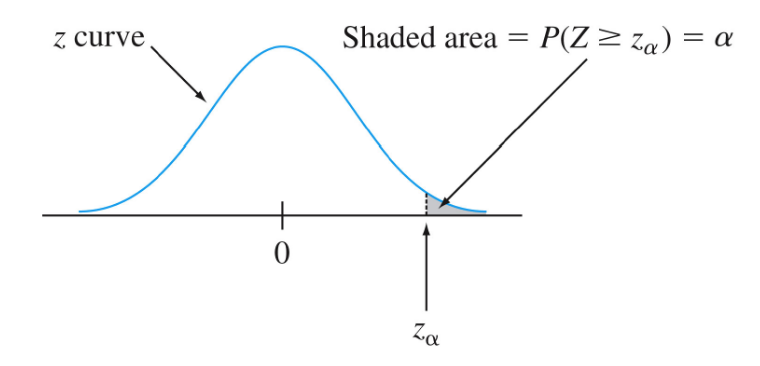
\includegraphics[scale=0.3]{1.png}
	\end{center}
}

\de{\b{Example 5.4 Contd.} From the diagram we see
	\begin{align*}
	\int_{y=2000}^{\infty} \int_{x=0}^{y} 6(10^{-6}\exp(-0.001x - 0.002y)) \, dx\, dy = 0.0500
	\end{align*}

}

\section{Independent Random Variables}

Recall that for independent events $E$ and $F$, the probability of $P(E \cap F) = P(E) P(F)$. Similarly if $X$ and $Y$ are random variable and independent if and only if
\begin{align}
P(X \in A, Y \in B) = P(X \in A) P(Y \in B)
\end{align}
In other words, any event involving $X$ is independent of any event involving $Y$. Also recall the following is true
\begin{align}
P(X \in A, Y \in B ) = f_{XY}(x,y) = f_X(x) f_Y(y) \text{ for all } x,y
\end{align}
Independence requires a rectangular range.

Independence depends on the physical situation being modelled and needs to be justified, for instance Binomial random variables require independent outcomes. Whereas the Hypergeometric has dependent outcomes.

\de{
\b{Example 5.11} This following example is the same as the previous, but we are going to modify the bounds to expand the rectangular region of integration. Notice the coefficient is smaller, this is due to the  larger bounds (total probability $\int_{0}^{\infty}\int_{0}^{\infty} f_{XY}(x,y) dx\, dy= 1$). 

Show that $X$ and $Y$ are independent and find $P(X > 1000, Y < 1000)$
\begin{align*}
f_{XY} = \begin{cases} 2(10^{-6}\exp(-0.001x - 0.002y)) & 0< x < \infty, 0 < y < \infty \\ 0 & else \end{cases}
\end{align*}

\b{Proof}
\begin{align*}
f_X = \int_{0}^{\infty} 2(10^{-6}\exp(-0.001x - 0.002y)) dy &= 0.001 e^{-0.001x}\\
f_Y = \int_{0}^{\infty} 2(10^{-6}\exp(-0.001x - 0.002y)) dx &= 0.002 e^{-0.002y}\\[2mm]
f_X f_Y  = 0.002\exp( - 0.002y) * 0.001 &e^{-0.001x} = f_{XY}
\end{align*}
Thus we have shown the variables are independent of each other
\begin{align*}
P(X > 1000, Y < 1000) &= P(X > 1000) P(Y < 1000)\\
&=	\int_{1000}^{\infty} 0.001 e^{-0.001x} \,dx \,\, \int_{0}^{\infty} 0.002 e^{-0.002y} \, dy\\
&= 0.3181
\end{align*}
}

\de{
	\b{Example 5.12} Suppose $(X,Y)$ are independent
	\begin{align*}
	X \thicksim N(10.5, 0.0025) \enspace Y \thicksim N(3.2, 0.0036)
	\end{align*}
	Find $P(10.4 < X < 10.6, 3.15 < Y < 3.25)$
	\\
	
	\b{Ans.}
	\begin{align*}
	P &= P(10.4 < X < 10.6)P(3.15 < Y < 3.25)\\
	&= P\bigg(\frac{10.4 - 10.5}{\sqrt{0.0025}} < Z < \frac{10.6 - 10.5}{\sqrt{0.0025}}\bigg) P\bigg(\frac{3.15 - 3.2}{\sqrt{0.0036}}< Z < \frac{3.25 - 3.2}{\sqrt{0.0036}}\bigg)\\
	&= P(-2 < Z < 2 ) P(-0.837  < Z < 0.833)\\
	&= ( P(Z < 2) - P(Z < -2) ) ( P( Z < 0.833) - P( Z < -0.837))\\
	&= 0.586
	\end{align*}
}

\end{document}